% --------------------------------------------------------------------------
% Template for DCASE 2019 technical reports; to be used with:
%          dcase2019_techrep.sty  - DCASE 2019 LaTeX style file, and
%          IEEEbib.bst - IEEE bibliography style file.
% Adapted from spconf.sty and waspaa15.sty
% --------------------------------------------------------------------------

\documentclass{article}
\usepackage{dcase2019_techrep,amsmath,graphicx,url,times,booktabs, tabularx}

% Example definitions.
% --------------------
\def\defeqn{\stackrel{\triangle}{=}}
\newcommand{\symvec}[1]{{\mbox{\boldmath $#1$}}}
\newcommand{\symmat}[1]{{\mbox{\boldmath $#1$}}}

% Title.
% --------------------
\title{URBAN SOUND TAGGING USING CONVOLUTIONAL NEURAL NETWORKS}

% Single addresses (uncomment and modify for single-address case).
% --------------------
% \name{Author(s) Name(s)\thanks{Thanks to XYZ agency for funding.}}
% \address{Author Affiliation(s)}
%
% For example:
% ------------
% \address{School\\
%       Department\\
%       Address}

% Two addresses
% --------------------

\name{Sainath Adapa}
\address{FindHotel\\
    Amsterdam, Netherlands \\
     adapasainath@gmail.com}


\begin{document}

\ninept
\maketitle

\begin{sloppy}

\begin{abstract}
This technical report outlines our solution to Task 5 of the DCASE 2019 challenge, titled \textit{Urban Sound Tagging}. The objective of the task is to label different sources of noise from raw audio data. A modified form of MobileNetv2, a convolutional neural network (CNN) model was trained to label both coarse and fine tags jointly. The proposed model uses log-scaled Mel-spectrogram as the representation format for the audio data. Mixup, Random erasing, scaling, and shifting are used as data augmentation techniques. A second model that uses scaled labels was built to account for human errors in the annotations. The solution code is available on GitHub\footnote{https://github.com/sainathadapa/urban-sound-tagging}.
\end{abstract}

\begin{keywords}
sound event detection (SED), machine listening, audio tagging, convolutional neural networks
\end{keywords}

\section{Introduction}
\label{sec:intro}

The Detection and Classification of Acoustic Scenes and Events (DCASE) \cite{dcase2019web}, now in its fifth edition, is a recurring set of challenges aimed at developing computational scene and event analysis methods. In Task 5, Urban Sound Tagging, the objective is to predict the presence or absence of 23 different types of noise sources in audio recordings. The 23 \textit{fine-grained} tags are further grouped into a list of 7 \textit{coarse-grained} tags. This hierarchical relationship is illustrated in Figure \ref{fig:taxonomy}.

For this challenge, SONYC \cite{bello2018sonyc} has provided 2351 recordings as part of the \textit{train} set, and 443 recordings as a part of the \textit{validate} set. All the recordings are ten seconds in length. Each recording was annotated by three Zooniverse\footnote{https://www.zooniverse.org/} volunteers. Additional annotations, specifically for \textit{validate} set, were performed by the SONYC team members and ground truth is then agreed upon by the SONYC team.

\begin{figure}[h]
\centering
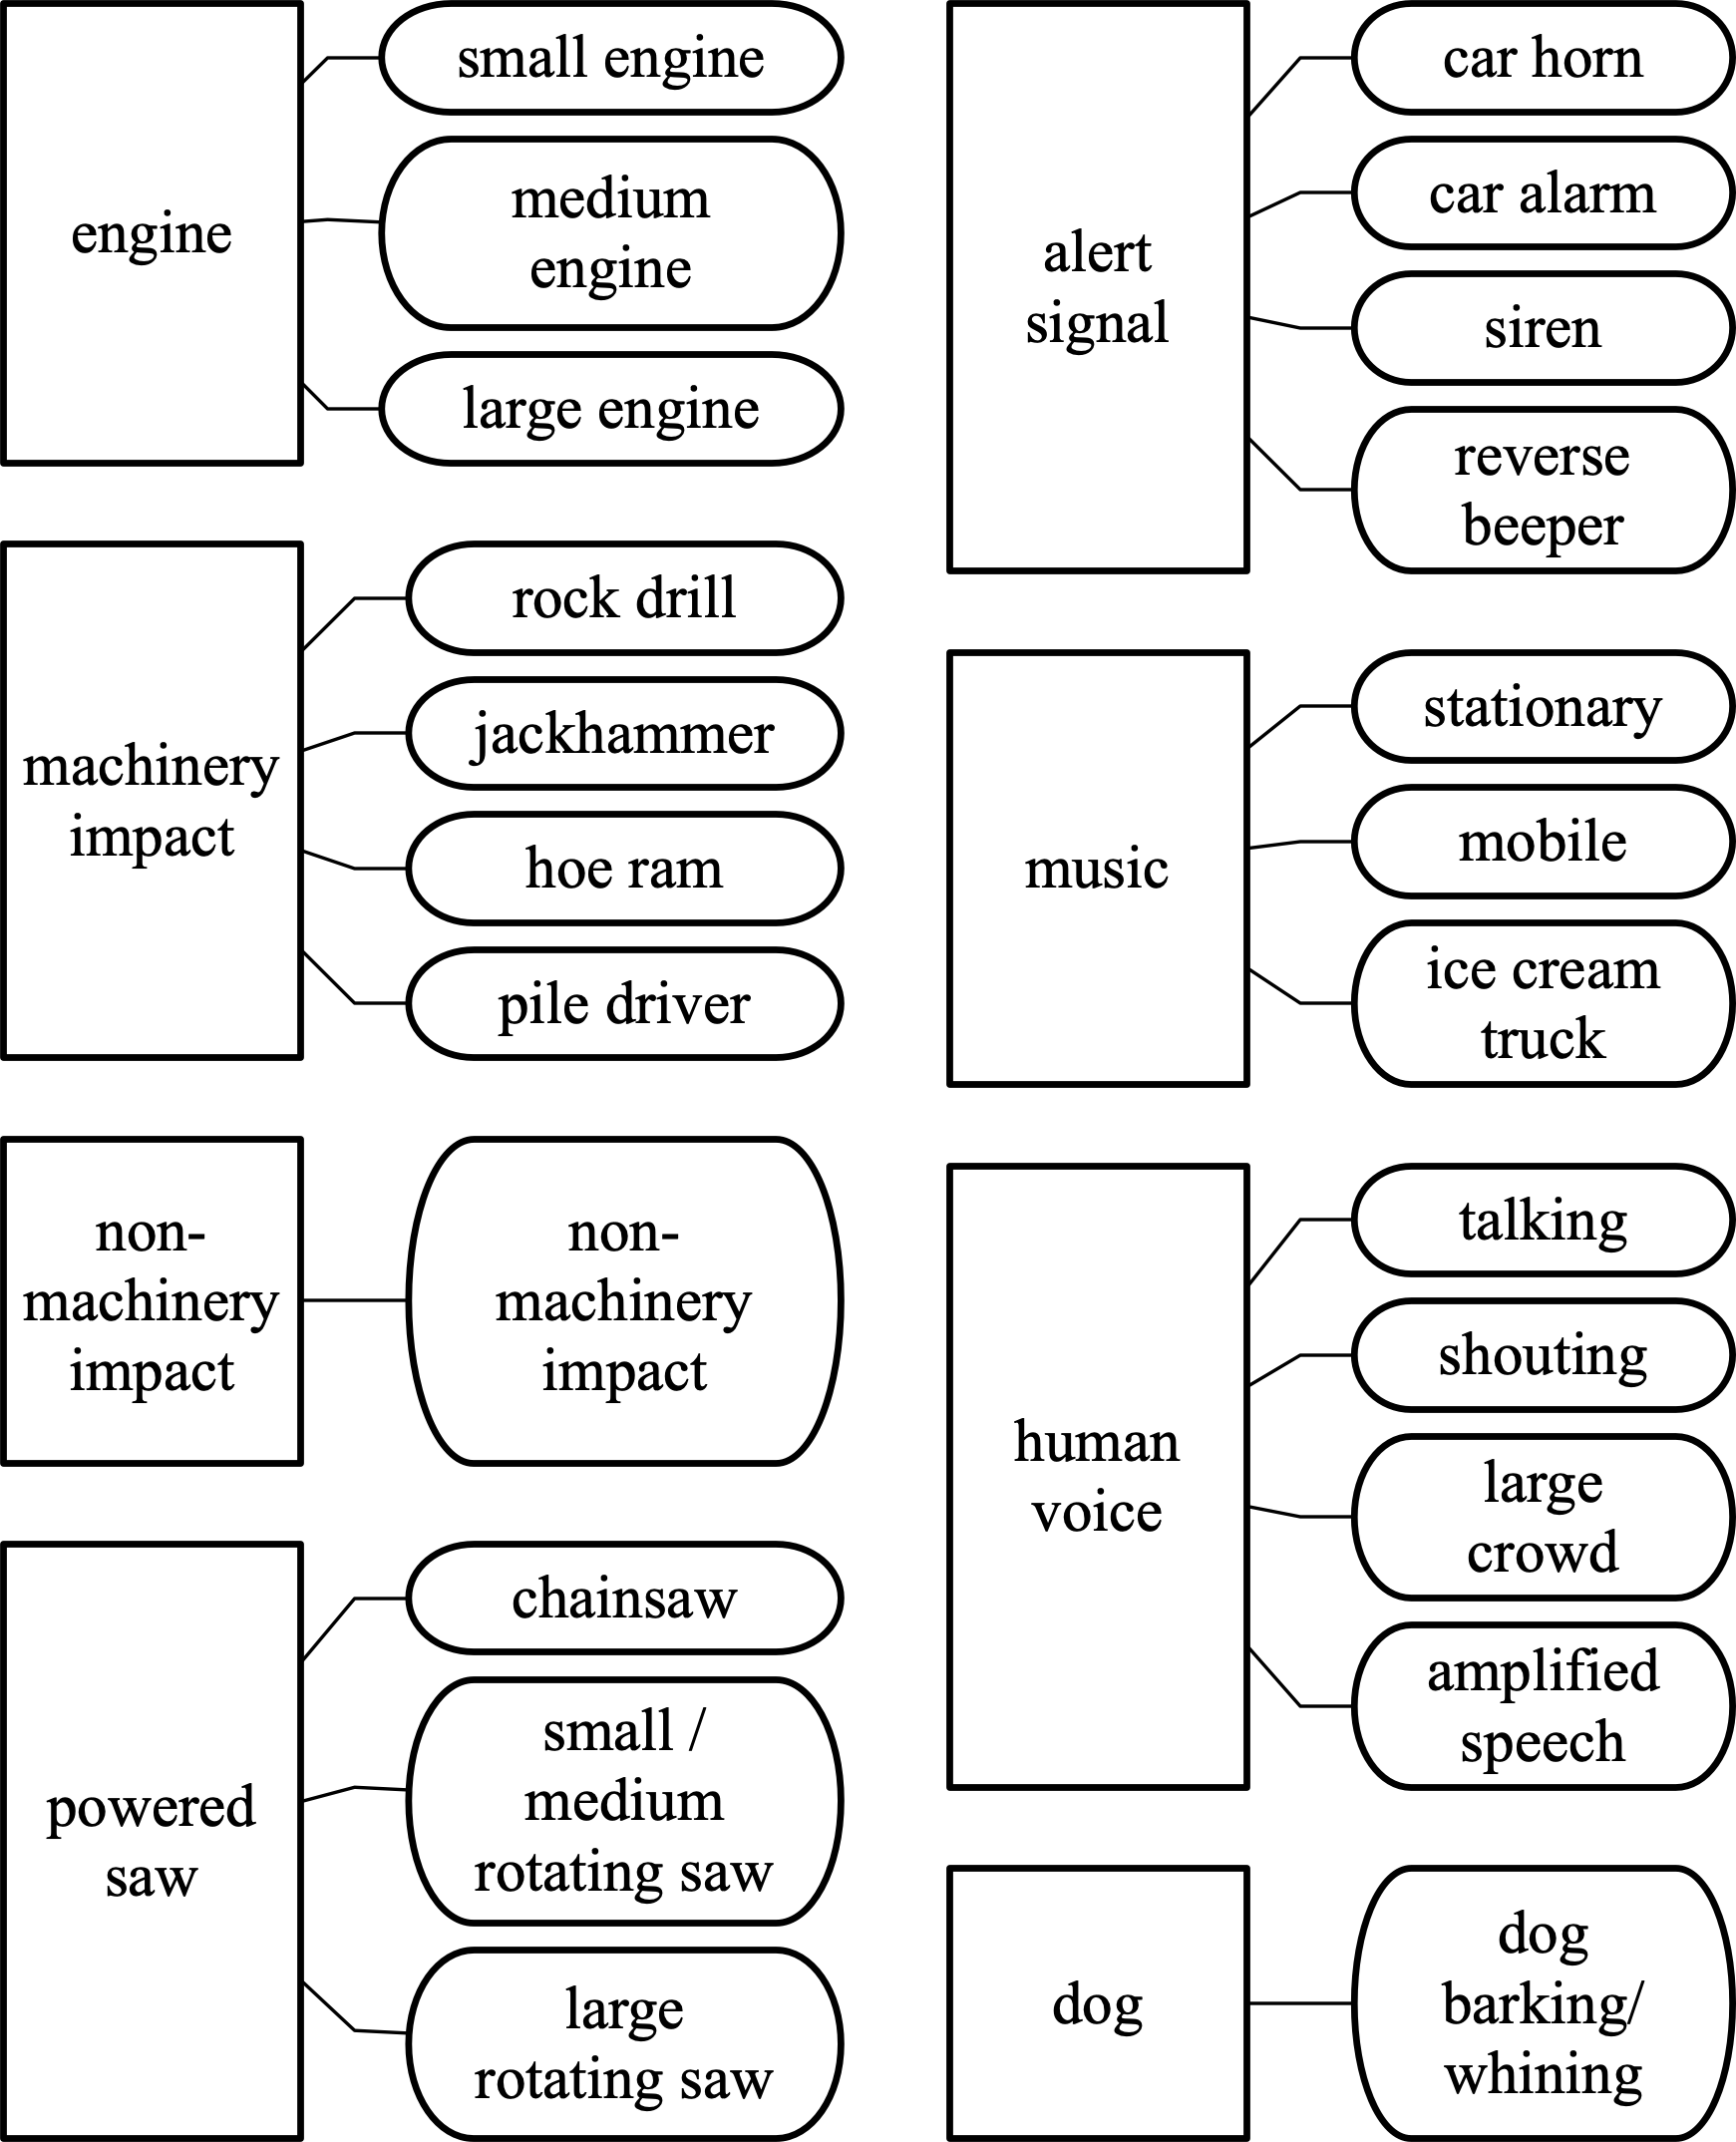
\includegraphics[scale=0.45]{task5_urban_sound_tagging.png}
\caption{Hierarchical taxonomy of tags. Rectangular and round boxes respectively denote coarse and fine tags. \cite{dcase2019task5}}
\label{fig:taxonomy}
\end{figure}

\section{Proposed framework}
\label{sec:framework}

\subsection{CNN Architecture}
\label{ssec:architecture}

\begin{table}
\centering
    \begin{tabular}{c|c|c}
    Input & Operator & Output\\
    \toprule
    $h \times w \times k$ & 1x1 \conv, \relus & $h \times w \times (tk)$\\
    $h \times w \times tk$& 3x3 \depthwise s=$s$, \relus & $\frac{h}{s} \times \frac{w}{s} \times (tk)$\\ 
    $\frac{h}{s} \times \frac{w}{s} \times tk$ & linear 1x1 \conv & $\frac{h}{s} \times \frac{w}{s} \times k'$\\
    \toprule
    \end{tabular}
    \caption{{\em Bottleneck residual block} transforming from $k$ to $k'$ channels, with stride $s$, and expansion factor $t$.}
\label{fig:bottlenec_block_table}
\end{table}

Convolutional neural network (CNN) based architectures have been proven to be useful for audio classification \cite{hershey2017cnn, salamon2017deep}. In this work, we use a modified form of MobileNetV2 \cite{sandler2018mobilenetv2}. The architecture of MobileNetV2 contains a 2D convolution layer at the beginning, followed by 19 \textit{Bottleneck residual blocks} (shown in Table \ref{fig:bottlenec_block_table}). Spatial average of the output from the final residual block is computed and used for classification via a linear layer.

The proposed model contains few modifications to the above-described architecture. The input Log Mel-spectrogram data is sent to the MobileNetV2 after first passing the input through two convolution layers. This is so that the single channel input can be converted into a three channel input. Instead of the spatial average, Max pooling is applied on the output from the final residual block. Additionally, the single linear layer at the end is replaced by two linear layers. The full architecture is described in Table \ref{mobilenet:arch}.

All the unmodified layers are initialized with weights from the MobileNetV2 model trained on ImageNet \cite{mv2weights}. Kaiming initialization \cite{he2015delving} is used for the remaining layers.


\subsection{Preprocessing and Data augmentation}
\label{ssec:preprocessing}

The proposed model uses Log Mel-spectrogram as the representation format for the input data. Librosa \cite{brian_mcfee_2019_2564164} toolbox was used to compute the Mel-spectrogram. For the Short-time Fourier transform (STFT), window size of 256 and hop length of 694 was used. For the Mel-frequency bins computation, lowest frequency and highest frequency of 20Hz and 22050Hz was used, with the number of bins being 128\footnote{https://www.kaggle.com/daisukelab/fat2019\_prep\_mels1}. No re-sampling or additional preprocessing steps were performed.

Several data augmentation techniques were used to supplement the training data. Deformations such as Time stretching and Pitch shifting that were previously shown to help in sound classification were employed \cite{salamon2017deep}. In addition, image augmentation methods such as Random rotate, Grid distortion \cite{2018arXiv180906839B}, and Random erasing \cite{zhong2017random} were used. Mixup \cite{zhang2017mixup}, an approach that linearly mixes two random training examples was used as well.

\begin{table}[]
\centering
\vspace{0pt}
\begin{tabular}{c|c|c|c|c}
Operator & $t$ & $c$ & $n$ & $s$ \\ \hline
\textbf{conv2d} & \textbf{-} & \textbf{10} & \textbf{1} & \textbf{1} \\
\textbf{conv2d} & \textbf{-} & \textbf{3} & \textbf{1} & \textbf{1} \\
conv2d & - & 32 & 1 & 2 \\
bottleneck & 1 & 16 & 1 & 1 \\
bottleneck & 6 & 24 & 2 & 2 \\
bottleneck & 6 & 32 & 3 & 2 \\
bottleneck & 6 & 64 & 4 & 2 \\
bottleneck & 6 & 96 & 3 & 1 \\
bottleneck & 6 & 160 & 3 & 2 \\
bottleneck & 6 & 320 & 1 & 1 \\
conv2d 1x1 & - & 1280 & 1 & 1 \\
\textbf{maxpool} & \textbf{-} & \textbf{1280} & \textbf{1} & \textbf{-} \\
\textbf{linear} & \textbf{-} & \textbf{512} & \textbf{1} & \textbf{-} \\
\textbf{linear} & \textbf{-} & \textbf{k} & \textbf{1} & \textbf{-} \\ \hline
\end{tabular}
\caption {Each line describes a sequence of 1 or more identical (modulo stride)  layers, repeated $n$ times. All layers in the same sequence have the same number $c$ of output channels. The first layer of each sequence has a stride $s$ and all others use stride $1$. All spatial convolutions use $3\times 3$ kernels (except for the first two which use $1\times 1$ kernels). The expansion factor $t$ is always applied to the input size as described in Table~\ref{fig:bottlenec_block_table}. Modifications to the MobileNetV2 architecture are highlighted in bold.}
\label{mobilenet:arch}
\end{table}

\section{Re-labeling}
\label{sec:relabeling}

For the \textit{validate set}, we have access to both the ground truth and the three annotations by Zooniverse volunteers. When the ground truth of a label is positive, 36\% of annotations (by Zooniverse volunteers) do not match with the ground truth. If the quality of the labels can be improved, it is quite possible that the accuracy of the model can be improved as well. Hence, a logistic regression model that takes the annotations as input and estimates the ground truth label was developed. This model was trained on the \textit{validate} set and then the ground truth estimate for the \textit{train set} were generated. Table \ref{fig:relabeleg} shows some predictions from the model.

\begin{table}[]
\centering
\begin{tabular}{cccc}
\hline
\begin{tabular}[c]{@{}c@{}}Coarse\\ label\end{tabular} & \begin{tabular}[c]{@{}c@{}}Fine\\ label\end{tabular} & \begin{tabular}[c]{@{}c@{}}Positive\\ annotations\\ count\end{tabular} & \begin{tabular}[c]{@{}c@{}}Predicted\\ score\end{tabular} \\ \hline
music & uncertain & 1 & 0.10 \\
music & uncertain & 3 & 0.98 \\
music & stationary & 2 & 0.88 \\
powered saw & chainsaw & 3 & 0.98 \\
machinery impact & - & 0 & 0.05 \\ \hline
\end{tabular}
\caption{Predictions for few cases from the automatic re-labeling model}
\label{fig:relabeleg}
\end{table}

\section{Training}

Two models were trained for this challenge:
\begin{itemize}
\item The first model generates probabilities for both the fine and coarse labels. During training, whenever the annotation is "unknown/other", loss for the fine tags corresponding to this coarse tag was masked out. Hence, this model does not generate predictions for the \textit{uncertain} fine labels. For each training example, loss is computed against each set of annotation separately. Average of the three loss values is taken as the loss value for this training example.
\item For the second model, predictions from the re-labeling model described in Section \ref{sec:relabeling} are used as labels. This model generates probabilities for both the fine and coarse labels, including the \textit{uncertain} fine labels.
\end{itemize}

Both the models use identical input data representation, and employ the same data augmentation techniques. They also use Binary Cross-entropy loss as the optimization metric. The models are trained on the \textit{train set} using the \textit{validate set} to determine the stopping point.

Training was done on PyTorch \cite{paszke2017automatic}. AMSGrad variant of the Adam algorithm \cite{kingma2014adam, reddi2019convergence} with a learning rate of 1e-3 was utilized for optimization. Whenever the loss on \textit{validate} set stopped improving for 5 \textit{epochs}, learning rate was reduced by a factor of 10. At the time of prediction, test-time augmentation (TTA) in the form of Time shifting was used.

\section{Results}
\label{sec:results}

The baseline system in \cite{dcase2019task5} computes VGGish embeddings \cite{hershey2017cnn} of the audio files, and builds a multi-label logistic regression on top of the embeddings. An additional baseline system that trains a CNN on the log Mel-spectrogram was described in \cite{kong2019cross}. Both the baseline systems count a positive for a tag if at least one annotator has labeled the audio clip with that tag. Table \ref{table:task5} shows the performance of the two baseline systems compared against the proposed models. It can be observed that re-labeling helped improve the Micro-AUPRC and the Micro-F1 metrics in case of Fine-grained labels.

\begin{table}
\centering
  \vspace{6pt}
  \centering
  \resizebox{\columnwidth}{!}{%
  \begin{tabular}{l p{0.8cm}p{0.8cm}p{0.8cm}p{0.8cm}p{0.8cm}p{0.8cm}}
    \toprule
    & \multicolumn{3}{c}{\textbf{\textsc{Fine-grained}}} & \multicolumn{3}{c}{\textbf{\textsc{Coarse-grained}}} \\
	\cmidrule(lr){2-4} \cmidrule(lr){5-7} 
	& \small{Micro AUPRC} & \small{Micro F1} & \small{Macro AUPRC} & \small{Micro AUPRC} & \small{Micro F1} & \small{Macro AUPRC} \\
	\midrule
 \begin{tabular}[c]{@{}l@{}}Baseline - 1\\ (VGGish \cite{dcase2019task5})\end{tabular} & 0.672 & 0.502 & 0.427 & 0.762 & 0.674 & 0.542 \\
 \begin{tabular}[c]{@{}l@{}}Baseline - 2\\ (CNN9-avg \cite{kong2019cross})\end{tabular} & 0.672 & 0.371 & 0.433 & 0.782 & 0.519 & 0.628 \\
 \begin{tabular}[c]{@{}l@{}}modified MobileNetV2\\ (no re-labeling)\end{tabular} & 0.772 & 0.489 & 0.594 & 0.861 & 0.602 & 0.702 \\
 \begin{tabular}[c]{@{}l@{}}modified MobileNetV2\\ (with re-labeling)\end{tabular} & 0.784 & 0.636 & 0.570 & 0.860 & 0.740 & 0.700 \\
	\bottomrule
\end{tabular}}
\caption{Performance on \textit{validate} set}
 \label{table:task5}
\end{table}

% -------------------------------------------------------------------------
% Either list references using the bibliography style file IEEEtran.bst
\bibliographystyle{IEEEtran}
\bibliography{refs}
%
% or list them by yourself
% \begin{thebibliography}{9}
% 
% \bibitem{dcase2016web}
%   \url{http://www.cs.tut.fi/sgn/arg/dcase2016/}.
%
% \bibitem{IEEEPDFSpec}
%   {PDF} specification for {IEEE} {X}plore$^{\textregistered}$,
%   \url{http://www.ieee.org/portal/cms_docs/pubs/confstandards/pdfs/IEEE-PDF-SpecV401.pdf}.
%
% \bibitem{PDFOpenSourceTools}
%   Creating high resolution {PDF} files for book production with 
%   open source tools, 
%   \url{http://www.grassbook.org/neteler/highres_pdf.html}.
%
% \bibitem{eWilliams1999}
% E. Williams, \emph{Fourier Acoustics: Sound Radiation and Nearfield Acoustic
%   Holography}. London, UK: Academic Press, 1999.
% 
% \bibitem{ieeecopyright}
%   \url{http://www.ieee.org/web/publications/rights/copyrightmain.html}.
%
% \bibitem{cJones2003}
% C. Jones, A. Smith, and E. Roberts, ``A sample paper in conference
%   proceedings,'' in \emph{Proc. IEEE ICASSP}, vol. II, 2003, pp. 803--806.
% 
% \bibitem{aSmith2000}
% A. Smith, C. Jones, and E. Roberts, ``A sample paper in journals,'' 
%   \emph{IEEE Trans. Signal Process.}, vol. 62, pp. 291--294, Jan. 2000.
% 
% \end{thebibliography}


\end{sloppy}
\end{document}
